%% The first command in your LaTeX source must be the \documentclass command.
\documentclass[acmtog]{acmart}
\usepackage[english,ngerman]{babel}
\usepackage[utf8]{inputenc} 

%% \BibTeX command to typeset BibTeX logo in the docs
\AtBeginDocument{%
  \providecommand\BibTeX{{%
    \normalfont B\kern-0.5em{\scshape i\kern-0.25em b}\kern-0.8em\TeX}}}
    
\copyrightyear{2024}
\acmYear{2024}
\citestyle{acmauthoryear}

\usepackage[figurename=Fig.]{caption}
\usepackage{csquotes}
\setcopyright{none}
\makeatletter
\renewcommand{\fnum@figure}{Abb. \thefigure}
\makeatother
\addto\captionsngerman{\renewcommand{\figurename}{Abb.}}
\settopmatter{printacmref=false} % Removes citation information below abstract
\renewcommand\footnotetextcopyrightpermission[1]{} % removes footnote with conference information in first column

%%
%% end of the preamble, start of the body of the document source.
\begin{document}

%%
%% The "title" command has an optional parameter,
%% allowing the author to define a "short title" to be used in page headers.
\title{Enterprise Architektur-Muster}

%%
%% The "author" command and its associated commands are used to define
%% the authors and their affiliations.
%% Of note is the shared affiliation of the first two authors, and the
%% "authornote" and "authornotemark" commands
%% used to denote shared contribution to the research.
\author{Julian Bruder}
\authornote{Alle Studierenden trugen zu gleichen Teilen zu dieser Arbeit bei.}
\author{Abdellah Filali}
\authornotemark[1]
\author{Luca Franke}
\authornotemark[1]
\affiliation{%
  \institution{Hochschule für Technik, Wirtschaft und Kultur Leipzig (HTWK Leipzig)}
  \streetaddress{Karl-Liebknecht-Str. 132}
  \city{Leipzig}
  %\state{Ohio}
  \country{Deutschland}
  \postcode{04277}
}
%%
%% By default, the full list of authors will be used in the page
%% headers. Often, this list is too long, and will overlap
%% other information printed in the page headers. This command allows
%% the author to define a more concise list
%% of authors' names for this purpose.
\renewcommand{\shortauthors}{Bruder, Filali, Franke}

%%
%% The abstract is a short summary of the work to be presented in the
%% article.
\begin{abstract}
Blah \ldots
\end{abstract}

\maketitle

\section{Einleitung}
% (Beschreibung von Kontext, Problemen, Anforderungen und Zielen)
Blah \ldots

\section{Grundlagen von Enterprise-Architekturen}
Blah \ldots

\section{Klassische Enterprise-Architekturen}
Blah \ldots

\section{Moderne Enterprise-Architekturen}

\subsection{Microkernel Architecture}\label{subsec:microkernel-architecture}
Die Microkernel Architecture ist ein Architekturmuster, was sich durch erweiterbarkeit, flexibilität und vor allem isolation der Funktionalitäten auszeichnet.
Wie in Abbildung~\ref{fig:microkernel} dargestellt, enthält ein Mikrokernel zwei wesentliche Komponenten: Den Kern der Anwendung,der die wichtigsten grundlegenden Funktionalitäten bereitstellt und Module oder auch Plugins,
die diesen Kern um Features und weitere Business Logik erweitern~\cite{architecturePatterns}.


\begin{figure}[!h]
  \centering
  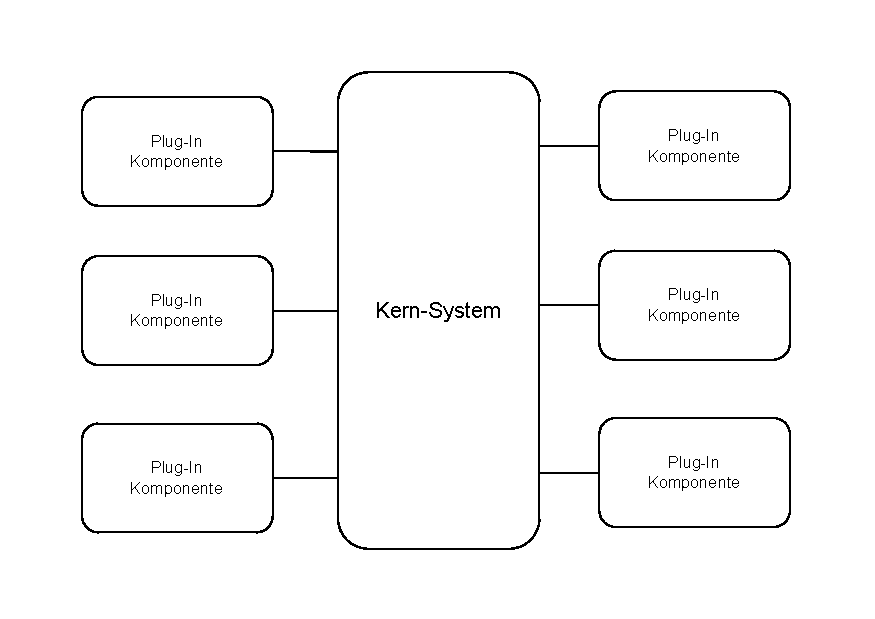
\includegraphics[width=\linewidth]{images/microkernel/microkernel}
  \caption{Aufbau einer Microkernel Architecture}
  \label{fig:microkernel}
\end{figure}

Der Kern der Anwendung implementiert dabei meist nur die minimalste Funktionalität, um die Anwendung oder das System lauffähig zu machen.
Alle weiteren Funktionalitäten werden in Modulen implementiert, die auf den Kern aufbauen.
Module sind meist unabhängig voneinander aufgebaut, es ist kann jedoch auch vorkommen, dass manche Module von anderen abhängig sind.
Dabei ist aber die best practice zu beachten, Kommunikation zwischen einzelnen Modulen so gering wie möglich zu halten, um Probleme durch Abhängigkeiten zu vermeiden.
Dadurch sind Module untereinander lose gekoppelt und können unabhängig voneinander entwickelt, getestet und deployed werden.

Die Plugins können über verschiedene Wege mit dem Kern verbunden werden.
Eine genaue Spezifikation zum Verbinden der Plugins mit dem Kern gibt es aber laut Architekturschema nicht, diese Entscheidung ist dem Entwickler überlassen und entsprechend der Anforderungen und Anwendungsumgebung zu treffen.
Beispielsweise könnte die Verbindung über Web-Services, Messaging oder am einfachsten über direkte Objekt-Instanziierung innerhalb der gleichen Anwendung stattfinden.

Zwischen Plugins und Kern werden Contracts definiert, die die Kommunikation zwischen den beiden Komponenten regeln.
Diese Standard Contracts können in Form von Interfaces, Klassen oder auch Datenstrukturen definiert werden.
Sollten Third Party Plugins zum Einsatz kommen, müssen sich diese an die definierten Contracts halten, um mit dem Kern kommunizieren zu können.
Alternativ können auch Adapter verwendet werden, um bestehende Plugins an den Kern bzw.\ die Contracts anzupassen.

Ein Problem, was sich durch diesen Aufbau ergibt, ist dass der Kern jederzeit wissen muss, welche Plugins aktuell verfügbar sind und wie diese angesprochen werden können.
Um dieses Problem zu lösen, kann eine Plugin-Registry verwendet werden.
Diese Registry enthält alle aktuell verfügbaren Plugins und die dazugehörigen relevanten Informationen wie z.B.\ Name des Service, Data Contracts, Verbindungsdetails, etc.
Der Kern der Anwendung kann dann zur Laufzeit auf diese Registry zugreifen und Plugins dynamisch laden.

Microkernel Architekturen können auch in anderen Architekturmustern eingebettet sein, falls es nicht möglich sein sollte die gesamte Software in diesem Architekturmuster aufzubauen.
Vor allem Teile von Anwendungen, die stark erweiterbar sein müssen, eignen sich gut für die Verwendung der Microkernel Pattern.

Ein klarer Vorteil dieses Architekturmusters ist die schnelle Reaktionsfähigkeit auf äußere Änderungen, da Anpassungen größtenteils nur in den isolierten Modulen vorgenommen werden.
Der Kern der Anwendung ist in den meisten Fällen schnell stabil und benötigt selten im Laufe der Entwicklung weitere Angleichungen.
Geänderte Module können je nach Implementierung auch zur Laufzeit geladen bzw.\ hinzugefügt werden, was mögliche Downtime von Software während des Entwicklungsprozesses minimiert.

Auch profitiert die Testbarkeit der Software durch die lose Kopplung der Module.
Jedes Modul kann unabhängig voneinander getestet werden und fehlende Module durch Mocks oder Stubs ersetzt werden, wodurch sich während der Entwicklung auf einzelne Funktionalitäten konzentriert werden kann.


\subsection{Event-Driven Architecture}
Die Event-Driven Architecture wählt als Basis einen anderen Ausgangspunkt als die bisherigen Architekturmuster.
Während bei letzteren Komponenten Dienste bereitstellen, welche von anderen Komponenten explizit genutzt werden,
verhalten sich Dienst-bereitstellende Komponenten in der Event-Driven Architecture reaktiv,
werden also implizit von Dienst-konsumierenden Komponenten genutzt \cite{garlanShawImplizit}.
Ein System reagiert somit asynchron auf Zustandsänderungen, also Ereignisse in diesem System \cite{eda}.
Die in dieser Architektur minimalen Einheiten, welche Informationen einer Zustandsänderung kapseln, werden \textit{Events} genannt.
Die Idee der impliziten Behandlung von Ereignissen ist nicht neu und taucht erstmals 1994 im von Garlan und Shaw publizierten Papier
\textit{\enquote{An introduction to Software Architecture}} auf.

Betrachten wir im Folgenden die Basis-Bestandteile der Event-Driven Architecture:
\begin{itemize}
  \item Ereignis (englisch \textit{Event}): Kapselt Information einer Zustandsänderung eines Systems
  \item Produzent (englisch \textit{Producer}): Komponente, die Event erzeugt
  \item Herausgeber (englisch \textit{Publisher}): Komponente, die, von Produzenten erzeugte, Events publiziert
  \item Konsument (englisch \textit{Consumer}): Reagiert auf publizierte Events
  \item Vermittler (englisch \textit{Mediator}): Liegt zwischen Produzenten und Konsumenten - filtert Events und verteilt diese auf Konsumenten
  \item Event-Bus: Oft auch \textit{Event-Broker} genannt - bietet die Infrastruktur für die Gesamtheit der Vermittler
\end{itemize}
Abstrakt kann ein Event als ein Vertrag zwischen Produzenten und Konsumenten am Event-Bus betrachtet werden.
Der Konsument nutzt die Spezifikation des Events am Bus, der Produzent implementiert jene Spezifikation.
Abbildung \ref{fig:eda} stellt diesen Vertrag dar.

\begin{figure}[!h]
  \centering
  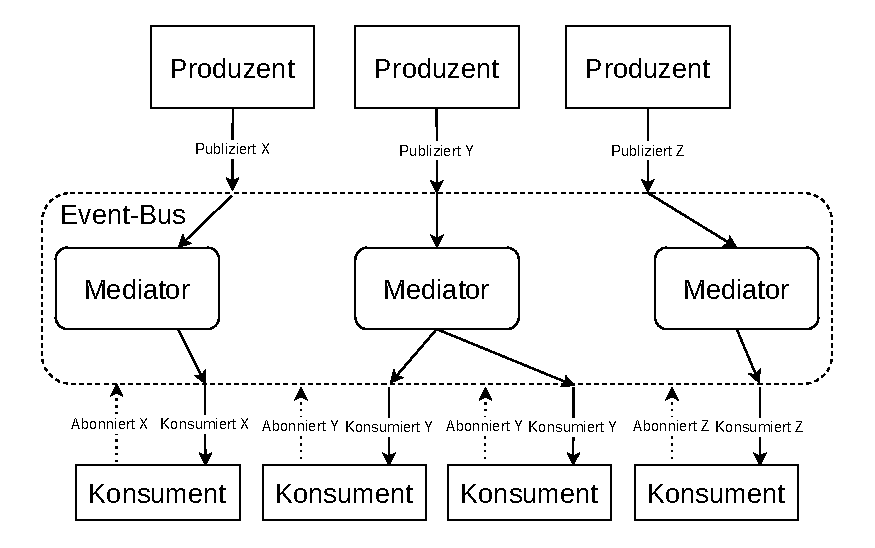
\includegraphics[width=\linewidth]{images/eda/eda.drawio}
  \caption{Vertrag zwischen Produzenten und Konsumenten am Event-Bus}
  \label{fig:eda}
\end{figure}

Durch den Vertrag weisen die Events am Event-Bus starke Kohäsion und somit lose Kopplung auf.
Diese lose Kopplung minimiert nicht nur kaskadierende Fehler, sondern ermöglicht agilen Entwickler-Teams durch klar abgegrenzte Features einfach definierbare Iterationen
- eine Menge von Events, deren Erzeugung und Konsumierung.

Weiter sind Events oft nah an dem, was Ereignisse in realen Prozessen sind, also domain-driven.
Gebündelt ermöglichen obige Punkte die kontinuierliche Auslieferung von Software in kurzen Intervallen.

Außerdem garantiert die asynchrone Behandlung von Ereignissen zusammen mit der loosen Kopplung maximale Skalierung.
Daher sind Event-Driven Architekturen besonders für datenintensive Echtzeit-Anwendungen wie IoT (Internet of Things) und Analytics geeignet \cite{iotEda}.

Die Agilität der Architektur kann weiter erhöht werden, indem der event-basierte Aspekt mit weiteren agilen Strukturen wie Microservices oder cloud-nativen Serverless-Functions kombiniert wird.
Die damit einhergehende Komplexität stellt teilweise hohe Anforderungen an die Entwickler.
Aufgrund der Asynchronität der Behandlung von Ereignissen ist die Testung des Systems meist schwer und die Fehlerbehandlung essentiell.
Mögliche Problemquellen schließen dabei unter anderem Event-Verlust, erhöhte Latenz und Inkonsistenz ein.
Die hohen Anforderungen an die Entwickler verlangen viel Vertrauen in jene, einer der zentralen Punkte des agilen Manifests \cite{agileManifesto}.
Insgesamt weist die Event-Driven Architecture also eine sehr hohe Agilität auf und ist damit besonders für moderne Software und ihre stetig wechselnden Anforderungen geeignet.

% TODO: Jetzt bestenfalls übergreifendes Beispiel

\section{Fallstudien und Praxisbeispiele}
Blah \ldots

\section{Diskussion}

\section{Zusammenfassung und Ausblick}
%(Überblick über die gesamte Arbeit, Rückführung auf Aussagen aus Kapitel 1 durchführen, offene Punkte als neue Forschungsfragen definieren)






\bibliographystyle{ACM-Reference-Format}
\bibliography{main}

\appendix

\section{Anhang 1}

\subsection{Übungsaufgaben}
Blah \ldots

\section{Anhang 2}
Blah \ldots

\end{document}
\endinput
